%=====================================================================
% COBRA-WATCH BE Major Project Report (RAIT D. Y. Patil Deemed to be University format)
% Compile order: pdflatex -> bibtex -> pdflatex -> pdflatex (Overleaf pdfLaTeX works natively)
%=====================================================================
\documentclass{RAITreport}

\usepackage{epsfig}
\usepackage{times}
\usepackage{graphicx}
\usepackage{amsmath,amssymb}
\usepackage{booktabs}
\usepackage{array}
\usepackage{url}
\usepackage[hidelinks]{hyperref}

\graphicspath{{./}{./figures/}}

\newtheorem{theorem}{Theorem}[chapter]
\newtheorem{assertion}[theorem]{Assertion}
\newtheorem{claim}[theorem]{Claim}
\newtheorem{conjecture}[theorem]{Conjecture}
\newtheorem{corollary}[theorem]{Corollary}
\newtheorem{definition}[theorem]{Definition}
\newtheorem{example}[theorem]{Example}
\newtheorem{figger}[theorem]{Figure}
\newtheorem{lemma}[theorem]{Lemma}
\newtheorem{prop}[theorem]{Proposition}
\newtheorem{remark}[theorem]{Remark}

\begin{document}

% Title page, Certificate, Approval, Declaration, Abstract, ToC, LoT, LoF
%=====================================================================
% prelude.tex — Title page, Certificate, Approval, Declaration, Abstract, ToC/LoT/LoF
%=====================================================================
\clearpage\pagenumbering{roman}

% [TODO — Confirm exact registered project title matching Review 1 submission]
\title{COBRA-WATCH: Passive Cyber-Physical Trust Scoring for Exposed Surveillance Cameras}

% Group members & roll numbers (confirm PRN/USN if college requires separate ID alongside Roll No)
\author{Aditya Ghadi (23CE1216)\\Aditya More (23CE1125)\\Akhade Kavtik (23CE1226)\\Ankita Devi (23CE1157)}

\setapprovalstudents{Aditya Ghadi (23CE1216), Aditya More (23CE1125), Akhade Kavtik (23CE1226), and Ankita Devi (23CE1157)}

\date{December 2026}

\project
\department{Department of Computer Engineering}

% [TODO — Confirm exact Prof. vs Miss styling with Vishakha Gaikwad & fill division coordinator name]
\setguide{Prof. Vishakha Gaikwad}
\setprojectcoordinatorname{[TODO: Name of Division Co-ordinator]}

\maketitle

\certificate
\makeapproval

\begin{declaration}
\begin{center}
\Large \bf {DECLARATION}
\end{center}
\noindent
I declare that this written submission represents my ideas and does not involve plagiarism. I have adequately cited and referenced the original sources wherever others' ideas or words have been included. I also declare that I have adhered to all principles of academic honesty and integrity and have not misrepresented or fabricated or falsified any idea/data/fact/source in my submission. I understand that any violation of the above will be cause for disciplinary action against me by the Institute and can also evoke penal action from the sources which have thus not been properly cited or from whom proper permission has not been taken when needed.
\end{declaration}

\begin{abstract}
Automated video surveillance pipelines routinely treat every incoming stream as authentic, while conventional IoT risk scanners score cameras purely from static vulnerability metadata. Consequently, an authenticated, patched device with zero known vulnerabilities can be subverted through a swapped decoy endpoint, a downscaling Man-in-the-Middle relay, or a looped video feed and still earn maximum trust. This project presents \textbf{COBRA-WATCH}, a strictly passive cyber-physical trust scoring system implementing \emph{Integrity-Gated Dual-Channel Trust Fusion} (IG-DCTF). Channel~A evaluates vulnerability posture $T_{\mathrm{cve}} \in [0, 100]$ from authentication flags, NVD/CISA KEV vulnerability classes, ownership inference, patch staleness, and multi-camera spatial corroboration. Channel~B quantifies signal authenticity $s \in [0, 1]$ by combining passive Tier~1 banner drift with Tier~2 visual frame liveness (\texttt{FrameLivenessTracker}). Both channels combine multiplicatively through a piece-wise Integrity Gate $T_{\mathrm{final}} = \mathrm{round}(T_{\mathrm{cve}} \cdot G(s))$ that hard-caps corrupted feeds at $T_{\mathrm{final}} \le 30$ (\texttt{low\_trust}) whenever $s < 0.50$.

Under an explicit passive-only legal boundary (zero outbound network probing to third-party hosts, zero raw IP redistribution, and whitelisted local footage only), real aggregate exposure analysis over Censys Platform metadata documents \textbf{104,218} exposed Indian camera hosts (\textbf{81,285} exposing RTSP port~554). On real public CUHK Avenue surveillance videos with controlled tamper injection, the tuned Tier~2 detector (\texttt{v2}) raises replay-loop detection on held-out test footage ($n = 16$ clips) from \textbf{1/16} (\textbf{6.2\%}) to \textbf{15/16} (\textbf{93.8\%}), achieves \textbf{16/16} detection across freeze, abrupt blur, gradual blur, full occlusion, partial occlusion, camera movement, and downscaling, reduces clean false alarms at the \texttt{tripped} tier to \textbf{0.0/h} ([0.0, 30.9], $0.1195$~h clean video), and executes at \textbf{242.7~FPS} ($320$~px) and \textbf{59.9~FPS} ($640$~px) on real decoded Avenue frames on an Intel Core i5-12450H CPU. An anonymized FastAPI and Next.js~16 operator console (\texttt{9,320} simulated \texttt{/24}-masked fixtures in \texttt{data/public.db}) demonstrates interactive gate exploration, live demo alert replay, and SHA-256 Merkle audit verification. Longitudinal Tier~1 historical drift and physical laboratory camera trials remain explicitly outside Review~2 scope as future work.
\end{abstract}

\tableofcontents
\listoftables
\listoffigures

\cleardoublepage\pagenumbering{arabic}


% Technical Chapters
\chapter{Introduction}

\section{Overview}\label{sec:intro_overview}
Networked surveillance cameras are increasingly wired directly into automated analytics workflows: person and perimeter detectors such as YOLOv8~\cite{jocher2023yolov8} and ByteTrack~\cite{zhang2022bytetrack} inspect frames and emit operational alerts, dispatch systems triage incidents across neighbouring devices, and forensic logs archive events for review. Throughout this pipeline sits an unexamined trust assumption---namely, that if an endpoint's software profile appears free of critical Common Vulnerabilities and Exposures (CVEs) and responds on its configured port, the video frames arriving from that device faithfully represent the live physical scene.

COBRA-WATCH addresses the resulting cyber-physical gap through \textbf{Integrity-Gated Dual-Channel Trust Fusion} (IG-DCTF). Instead of collapsing all trust into vulnerability counts, COBRA-WATCH separates \emph{vulnerability posture} (Channel~A, $T_{\mathrm{cve}} \in [0, 100]$) from \emph{signal authenticity} (Channel~B, $s \in [0, 1]$) and couples them through a multiplicative gate $T_{\mathrm{final}} = T_{\mathrm{cve}} \cdot G(s)$. When a feed fails physical or protocol liveness checks ($s < 0.50$), the gate floor ($G = 0.30$) caps the final score at $T_{\mathrm{final}} \le 30$ (\texttt{low\_trust}) regardless of how clean Channel~A looks. All exposure analysis operates strictly passively on aggregate search metadata, and visual analysis executes strictly offline on local or public benchmark video without ever opening unauthorized remote Real-Time Streaming Protocol (RTSP) streams.

\section{Motivation}
Internet-exposed surveillance infrastructure presents both massive cyber-posture exposure and asymmetric physical deception risk. Public scan metadata indexed by search engines such as Shodan~\cite{matherly2015shodan} and Censys routinely surfaces hundreds of thousands of unmanaged embedded camera interfaces, many vulnerable to Mirai-class credential brute-forcing~\cite{antonakakis2017mirai,griffioen2020mirai} or vendor firmware flaws~\cite{das2022kalay}. In a non-attributive aggregate snapshot collected under Censys research access (Ticket RS-469; \texttt{data/censys/2026-11-26/snapshot.json}), the query \texttt{host.location.country: "India" AND host.services.hardware.type: "CAMERA"} returned \textbf{104,218} exposed Indian camera hosts across six aggregate telemetry dimensions, with \textbf{81,285} hosts advertising unencrypted or exposed RTSP service port~554.

At the same time, security-only defenses address only half the threat surface. Suppose two identical IP cameras declare the same HTTP server banner, firmware version, and clean CVE catalog ($T_{\mathrm{cve}} = 100$). An attacker who replaces one endpoint behind a proxy with a replayed video loop, degrades optical sharpness gradually, occludes part of the lens, or proxies a lower-resolution stream leaves vulnerability metadata completely unchanged. Pure CVE scorers rate both feeds equally trustworthy, forwarding tampered alarms into automated dispatch queues. Bridging cyber-posture intelligence with signal liveness checks motivates the dual-channel IG-DCTF architecture.

\section{Problem Statement and Objectives}
\subsection*{Problem Statement}
Given heterogeneous passive camera posture metadata and optional authorized video frame streams, single-channel vulnerability trust scorers cannot detect spoofed, relayed, frozen, looped, blurred, occluded, or resolution-downgraded feeds, allowing malicious or tampered feeds from nominally secure devices to trigger high-trust alerts.

\subsection*{Objectives}
The project targets four verifiable engineering objectives within a strict passive ethics and legal boundary (India's IT Act, 2000 \S43/\S66 and DPDP Act, 2023):
\begin{enumerate}
  \item \textbf{IG-DCTF Scoring and Hard Integrity Gating:} Formulate and implement a dual-channel scoring engine with a piece-wise multiplicative gate ($\theta_{\mathrm{low}} = 0.50$, $\theta_{\mathrm{high}} = 0.85$, floor $0.30$, hard cap $30$) ensuring non-compensation for compromised signal integrity while preserving tolerance for benign single-field firmware drift.
  \item \textbf{Real-Video Tier~2 Tamper Detection (\texttt{v2}):} Build and validate \texttt{FrameLivenessTracker} capable of flagging freezes, natural-motion replay loops, abrupt/slow blur, full/partial lens occlusion, camera displacement, and resolution downgrades at real-time CPU speeds on public CUHK Avenue surveillance footage.
  \item \textbf{Passive Metadata Integration and Forensic Auditability:} Collect aggregate Censys exposure counts without storing or publishing raw target IP addresses, persist API alert decisions in an idempotent SHA-256 Merkle-chained ledger (\texttt{audit\_ledger}), and permanently prohibit active outbound host probing.
  \item \textbf{Interactive Console and Experimental Transparency:} Deliver an anonymized FastAPI + Next.js~16 operator console (\texttt{/console}, \texttt{/lab}, \texttt{/research}, \texttt{/ethics}) that enforces \texttt{/24} IP masking and explicitly separates real public metrics from labelled demo fixtures (\texttt{data/public.db}, $n = 9,320$ simulated devices) and counterfactual formula checks ($n = 120$).
\end{enumerate}

\section{Organization of the Report}
The remainder of this report follows the standard structure. Chapter~2 reviews prior literature across IoT compromise measurement, camera CVE assessment, trust-fusion models, and surveillance tamper detection, isolating the cyber-physical blind spot. Chapter~3 presents the passive threat model, IG-DCTF mathematical formulation, Tier~1/Tier~2 detectors, full-stack architecture, and software/hardware environment. Chapter~4 documents implementation workflows, automated unit/contract test suites, real Censys and CUHK Avenue evaluation results alongside CPU throughput benchmarks, and synthetic counterfactual ablation checks. Chapter~5 concludes the report with honest scope boundaries and future research directions.

\chapter{Literature Survey}

\section{Survey of Existing System}
Research relevant to trustworthy surveillance alerting spans four largely disconnected domains: empirical IoT compromise measurement, camera vulnerability auditing, multi-attribute trust scoring, and automated video tamper analytics.

\subsection{IoT Compromise and Exposure Measurement}
Foundational empirical studies demonstrate how rapidly exposed consumer and enterprise IP cameras fall under adversarial control. Antonakakis et al.~\cite{antonakakis2017mirai} reconstructed the global Mirai botnet outbreak, showing that default telnet/web credentials on embedded cameras and DVRs enable large-scale automated recruitment. Griffioen and Doerr~\cite{griffioen2020mirai} measured device turnover under active botnet competition on time scales spanning hours to days, while Zhang et al.~\cite{zhang2020forensics} and Famera et al.~\cite{famera2025mirai} documented Mirai variants and server-side forensic artifacts. Commercial banner indexing described by Matherly~\cite{matherly2015shodan} and platform telemetry from Censys make this public exposure observable at country scale. However, measurement studies describe population compromise rates; they do not evaluate individual alert reliability at dispatch time.

\subsection{Camera Vulnerability Assessment}
Dedicated camera security audits score device firmware and service exposure using public vulnerability databases such as NIST NVD~\cite{nvd}, EPSS exploit probabilities~\cite{jacobs2021epss}, and the CISA Known Exploited Vulnerabilities (KEV) catalog~\cite{cisakev}. Bernot et al.~\cite{bernot2025cctv} assessed China-made IoT cameras via CVSS vectors, Oliver~\cite{oliver2025ipcam} categorized IP-camera CVE patterns across NVD records, KTH researchers mapped public camera banners to known advisories~\cite{kth2018cameras}, and Auti et al.~\cite{auti2025vapt} proposed automated VAPT auditing scripts for CCTV and DVR appliances. These pipelines establish cyber risk posture ($T_{\mathrm{cve}}$), but remain blind to whether the physical camera stream is live or spoofed.

\subsection{IoT Trust and Reputation Models}
Comprehensive surveys~\cite{ferraris2024trust,iottrust2023slr,biot2026trust} organize IoT trust computation into weighted-average aggregators, Bayesian log-odds inference, graph-based reputation models, and game-theoretic formulations. Common hazards across deployed trust engines include susceptibility to collusive rating rings, Sybil node inflation, cold-start ambiguity for unseen hosts, and linear compensation where healthy metrics mask failing components. SCI-IoT~\cite{swami2025sciiot} addresses static certification using explicit critical gates; COBRA-WATCH extends that gating concept from procurement-time device evaluation into per-alert run-time gating over dynamic feed health. Graph Convolutional Networks~\cite{kipf2017gcn} offer structural detection for collusive corroboration graphs when topological labels exist.

\subsection{Automated Video Analytics and Tamper Primitives}
Modern surveillance stacks combine real-time object detection (YOLOv8~\cite{jocher2023yolov8}) and multi-object association (ByteTrack~\cite{zhang2022bytetrack}) for downstream tasks such as abandoned-object alerting~\cite{luna2018aod,yilmazer2025abandoned}, multi-camera loitering tracking~\cite{nayak2019loitering}, and scene anomaly detection~\cite{rasal2025suspicious,liu2025epipolar}. While vision systems rely on perceptual hashing~\cite{zauner2010phash} and focus sharpness metrics such as variance of the Laplacian~\cite{pech2000focus} for low-level tamper primitives, conventional alerting stacks process every decoded frame uniformly without conditioning dispatch confidence on either OSINT cyber posture or real-time cryptographic audit trails~\cite{merkle1987}.

\section{Limitations of Existing System or Research Gap}
Comparing representative systems across existing domains highlights a structural blind spot summarized in Table~\ref{tab:lit_gap}. Security scanners verify vulnerability posture without checking feed liveness, while computer-vision pipelines evaluate video content without consulting vulnerability, banner consistency, or tamper-evident audit chains.

\begin{table}[!ht]
  \centering
  \caption{Capability comparison across representative system classes}
  \label{tab:lit_gap}
  \begin{tabular}{@{}lcccc@{}}
    \toprule
    \textbf{Work Class} & \textbf{Vuln. Posture} & \textbf{Feed Authenticity} & \textbf{Fused Gate} & \textbf{Per-Alert Audit} \\
    \midrule
    Camera vuln. assessment~\cite{bernot2025cctv,oliver2025ipcam,auti2025vapt} & Yes & No & No & No \\
    IoT trust \& certification~\cite{swami2025sciiot,ferraris2024trust,biot2026trust} & Partial & No & No & No \\
    Video analytics \& tracking~\cite{jocher2023yolov8,zhang2022bytetrack,nayak2019loitering} & No & No & No & Yes \\
    \textbf{COBRA-WATCH (IG-DCTF)} & \textbf{Yes} & \textbf{Yes} & \textbf{Yes} & \textbf{Yes} \\
    \bottomrule
  \end{tabular}
\end{table}

Crucially, even hybrid scoring schemes that rely on simple additive combinations ($T_{\mathrm{cve}} - c(1-s)$) suffer from linear compensation: a camera with $T_{\mathrm{cve}} = 100$ subjected to an acute signal integrity drop can still retain sufficient points to land in \texttt{medium\_trust} or delay operator triage. Closing this cyber-physical gap requires (i) non-compensatory multiplicative gating tied to explicit threshold bounds, (ii) memory-efficient temporal loop and spatial occlusion detection that operates without ground-truth remote camera probing, and (iii) tamper-evident logging paired with transparent separation of real public telemetry from simulated console demonstration fixtures.

\chapter{Proposed System}

\section{Problem Statement and Passive Threat Model}
The objective of COBRA-WATCH is to compute a per-alert reliability score $T_{\mathrm{final}} \in [0, 100]$ and actionable tier (\texttt{high\_trust} $\ge 80$, \texttt{medium\_trust} $50\text{--}79$, \texttt{low\_trust} $< 50$) for surveillance alerts without violating legal privacy boundaries or sending intrusive traffic to third-party endpoints.

The system considers four concrete adversarial classes within an explicit passive boundary:
\begin{itemize}
  \item \textbf{Decoy Swapping or MITM Relay ($\mathcal{A}_1$):} An adversary substitutes a camera endpoint behind a reverse proxy or inserts a transcoding relay that lowers resolution or changes banner fingerprints while keeping a clean IP/CVE profile.
  \item \textbf{Stream Freeze or Replay Loop ($\mathcal{A}_2$):} An attacker stalls frame updates, injects pre-recorded looping video segments with realistic natural motion, degrades focus sharpness gradually, covers the lens partially/completely, or shifts camera orientation.
  \item \textbf{Collusive Corroboration ($\mathcal{A}_3$):} Compromised neighbouring devices fabricate rapid cross-camera event confirmations to inflate spatial trust bonuses.
  \item \textbf{API Metadata Spoofing ($\mathcal{A}_4$):} Tampered detection-event payloads attempt to overwrite stored vulnerability posture, replay old nonces, or flood the ingestion endpoint.
\end{itemize}

\textbf{Passive Measurement Constraint:} COBRA-WATCH never opens outbound sockets or TCP probes to external target cameras (legacy active heartbeat modules were permanently deleted from the codebase). OSINT intake uses aggregate search telemetry strictly without exporting target IP lists, and the video analysis subsystem rejects any non-whitelisted remote RTSP stream URI via \texttt{\_assert\_source\_is\_authorized()}.

\section{Proposed Methodology and Techniques}

\subsection{Channel A: Vulnerability Posture ($T_{\mathrm{cve}}$)}
For every indexed camera $d$, Channel~A computes a cyber-posture score $T_{\mathrm{cve}} \in [0, 100]$ strictly from server-side database attributes rather than client-supplied payload assertions:
\begin{equation}
  T_{\mathrm{cve}} = \mathrm{clip}_{[0, U]}\!\Big(100 - 30\,\mathbf{1}[\neg \mathrm{auth}] - \Delta_{\mathrm{cat}} - 20\,\mathbf{1}[\text{owner unknown}] - 15\,\mathbf{1}[\mathrm{stale}] - 10\,\mathbf{1}[\mathrm{lat} > 500] + \beta(k)\Big),
\end{equation}
where $U = 49$ if the camera allows unauthenticated stream access (otherwise $100$), $\Delta_{\mathrm{cat}} \in \{0, 15, 25, 30\}$ reflects CWE vulnerability classes mapped from NVD/CISA KEV/EPSS feeds~\cite{nvd,cisakev,jacobs2021epss}, and $\beta(k) \in \{-10, 0, +20\}$ captures spatial corroboration from $k$ nearby cameras ($k = 0, 1, \ge 2$) protected by velocity limits against collusion~\cite{kipf2017gcn}.

\subsection{Channel B, Tier 1: Passive Banner Drift}
Tier~1 derives a banner fingerprint $\mathcal{B}_d(t) = \langle \mathrm{firmware}, \mathrm{server}, \mathrm{ports}, \mathrm{resolution}, \mathrm{product}, \mathrm{codec}\rangle$ from passive metadata snapshots and computes weighted field divergence:
\begin{equation}
  \mathrm{Drift}(d, t) = \frac{\sum_{i} w_i\,\delta_i\big(\mathcal{B}_d(t)[i], \mathcal{B}_d(t-1)[i]\big)}{\sum_i w_i} \in [0, 1],
\end{equation}
with default field weights $w = (0.25, 0.20, 0.20, 0.20, 0.10, 0.05)$ aligned with firmware, HTTP server, open-port Jaccard set distance, resolution downgrade, product string, and codec changes, flagging drift anomalies above $0.15$. Because no single banner weight exceeds $0.25$, single-field updates produce a gentle taper rather than a false gate trip.

\subsection{Channel B, Tier 2: Visual Frame Liveness (\texttt{v2})}
For whitelisted local and dataset video sources, \texttt{FrameLivenessTracker} (\texttt{video\_pipeline/liveness\_detector.py}, \texttt{v2} frozen at commit \texttt{023c5c4}) inspects incoming frames along orthogonal checks summarized in Figure~\ref{fig:tier2_pipeline}:
\begin{enumerate}
  \item \textbf{Freeze and Replay-Loop Ring Buffer:} Each frame yields an un-smoothed \texttt{INTER\_NEAREST} $32 \times 32$ grayscale $8\times 8$ DCT perceptual hash~\cite{zauner2010phash}. Consecutive Hamming distances $d_t \le 1$ catch static freezes after $25$ frames, while a temporal ring buffer combined with prefix-sum pixel-motion verification catches replayed segments even when natural motion preserves frame-to-frame change. A static-scene variance guard suppresses false freeze alarms in genuine stationary scenes.
  \item \textbf{Sharpness Drift and Anchored Slow Blur:} Variance of the Laplacian $v_t$~\cite{pech2000focus} tracks both immediate focus drops against an EWMA baseline ($\mu_t = \alpha v_t + (1-\alpha)\mu_{t-1}, \alpha = 0.05$) and slow cumulative defocus relative to anchored initialization sharpness.
  \item \textbf{Partial Occlusion and Scene Displacement:} An $8 \times 8$ spatial variance/contrast block test flags partial lens coverage (\texttt{partial\_cover}), and coarse layout edge correlation identifies sudden camera displacement (\texttt{moved}).
  \item \textbf{Resolution Mismatch:} Frame resolution $(W \times H)$ is verified against the stream resolution declared in Tier~1 metadata.
\end{enumerate}

The combined liveness score takes weights $w = (1.0, 0.6, 0.5)$ motivated by single-factor gate reachability:
\begin{equation}
  L(t) = 1 - \max\big(1.0\,F_t,\, 0.6\,q_t,\, 0.5\,m_t\big) \in [0, 1].
\end{equation}

\begin{figure}[!ht]
  \centering
  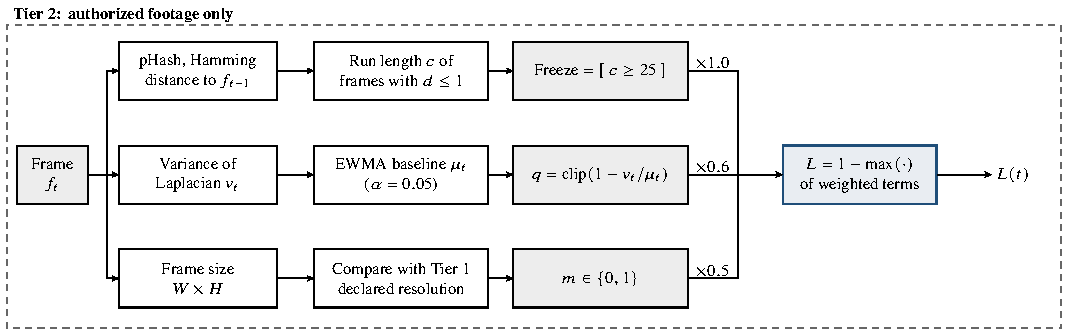
\includegraphics[width=0.92\textwidth]{fig05_tier2_liveness.pdf}
  \caption{Tier~2 frame liveness computation across perceptual-hash freeze/loop, Laplacian blur drift, and declared-resolution validation}
  \label{fig:tier2_pipeline}
\end{figure}

\subsection{Multiplicative Integrity Gate and Formal Guarantees}
Channel~B signal integrity combines both tiers via $s = (1 - \mathrm{Drift})\,L$ when Tier~2 is authorized (else $s = 1 - \mathrm{Drift}$), driving the piece-wise Integrity Gate $G(s)$ plotted in Figure~\ref{fig:gate_fn}:
\begin{equation}
  G(s) = \begin{cases}
    1, & s \ge \theta_{\mathrm{high}} = 0.85 \quad (\texttt{nominal}), \\[4pt]
    0.30 + 0.70\,\dfrac{s - 0.50}{0.85 - 0.50}, & 0.50 \le s < 0.85 \quad (\texttt{tapered}), \\[6pt]
    0.30, & s < \theta_{\mathrm{low}} = 0.50 \quad (\texttt{hard\_gated}),
  \end{cases}
  \qquad T_{\mathrm{final}} = \mathrm{round}\big(T_{\mathrm{cve}}\,G(s)\big).
\end{equation}
When $s < 0.50$, the gate enforces an explicit floor multiplier of $0.30$ and hard cap of $T_{\mathrm{final}} \le 30$. This satisfies three core properties: (i) \emph{non-compensation} (a pristine $T_{\mathrm{cve}} = 100$ camera cannot avoid \texttt{low\_trust} once $s < 0.50$), (ii) \emph{single-field tolerance} (one Tier~1 banner bump produces $\mathrm{Drift} \le 0.25$ and stays above $0.50$), and (iii) \emph{Lipschitz sensitivity} with bounded slope $2\,T_{\mathrm{cve}}$ inside the taper zone.

\begin{figure}[!ht]
  \centering
  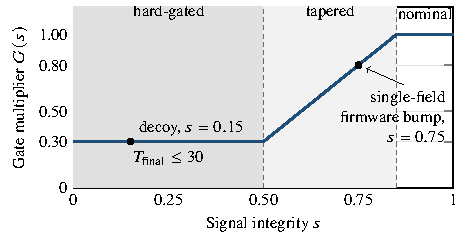
\includegraphics[width=0.72\textwidth]{fig06_gate_function.pdf}
  \caption{Multiplicative Integrity Gate $G(s)$ with thresholds $\theta_{\mathrm{low}} = 0.50$, $\theta_{\mathrm{high}} = 0.85$, floor $0.30$, and hard cap $30$}
  \label{fig:gate_fn}
\end{figure}

\section{System Design}
As illustrated in Figure~\ref{fig:arch}, COBRA-WATCH separates ingestion, scoring, and presentation across three containerized services:
\begin{itemize}
  \item \textbf{FastAPI Backend (\texttt{backend/}):} Implements REST and WebSocket endpoints (\texttt{/api/devices}, \texttt{/api/alerts}, \texttt{/api/detection-event}, \texttt{/api/ws/alerts}, \texttt{/api/censys/snapshots}, \texttt{/api/audit/*}, \texttt{/api/scenarios/run}, \texttt{/api/nl-query}) backed by SQLite with separate async/sync audit paths and $30$~s write lock timeouts. Admission controls (Figure~\ref{fig:event_pipeline}) verify constant-time \texttt{X-API-Key} authentication, 5-minute idempotency keys (HTTP~409), 10~events/min per-camera rate limits (HTTP~429), and a 60~s timestamp freshness window (HTTP~400) before persistence into the SHA-256 hash-chained \texttt{audit\_ledger}~\cite{merkle1987}. All public reads mask host octets to \texttt{/24} unless \texttt{EXPOSE\_FULL\_IP=true}.
  \item \textbf{Video AI Pipeline (\texttt{video\_pipeline/}):} Executes YOLOv8~\cite{jocher2023yolov8}, ByteTrack~\cite{zhang2022bytetrack}, spatial rule rules, and \texttt{FrameLivenessTracker} offline on whitelisted video files, pushing structured \texttt{visual\_liveness} alerts to \texttt{POST /api/detection-event}.
  \item \textbf{Next.js 16 Operator Web Application (\texttt{frontend/}):} Provides five primary routes: interactive IG-DCTF methodology overview (\texttt{/}), real-vs-synthetic research comparisons (\texttt{/research}), Gate Explorer + live WebSocket demo scenario runner (\texttt{/lab}), ethics disclosures (\texttt{/ethics}), and MapLibre GL JS triage console (\texttt{/console}) displaying self-hosted India boundaries with explicit \texttt{Simulated fixture} tags when connected to \texttt{data/public.db}.
\end{itemize}

\begin{figure}[!ht]
  \centering
  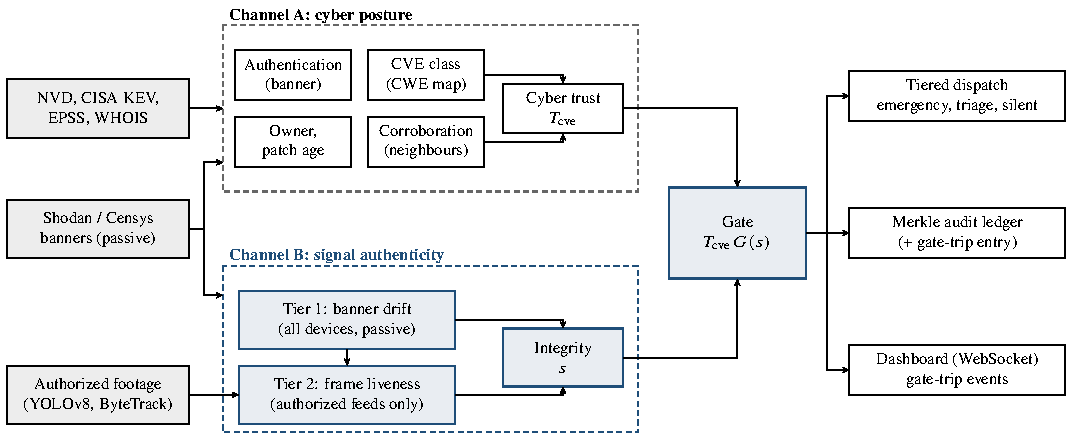
\includegraphics[width=0.95\textwidth]{fig02_architecture.pdf}
  \caption{COBRA-WATCH end-to-end passive cyber-physical architecture}
  \label{fig:arch}
\end{figure}

\begin{figure}[!ht]
  \centering
  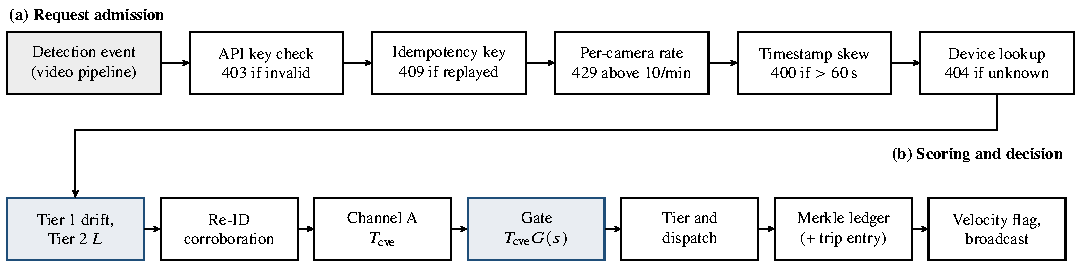
\includegraphics[width=0.95\textwidth]{fig07_event_pipeline.pdf}
  \caption{Detection event admission checks (API key, idempotency, rate limit, clock skew) prior to IG-DCTF scoring and Merkle ledger append}
  \label{fig:event_pipeline}
\end{figure}

\section{Details of Hardware and Software Requirements}
Table~\ref{tab:hw_sw} lists the verified development and evaluation stack used across Windows and Linux test hosts.

\begin{table}[!ht]
  \centering
  \caption{Hardware and software specifications}
  \label{tab:hw_sw}
  \begin{tabular}{@{}p{4.2cm}p{10.5cm}@{}}
    \toprule
    \textbf{Component} & \textbf{Specification} \\
    \midrule
    Evaluation Host & Intel Core i5-12450H CPU (CPU-only OpenCV / PyTorch inference benchmark); cross-tested on Windows~11 and Kali Linux \\
    Memory \& Storage & 16~GB RAM recommended for local Next.js~16 dev/build + YOLOv8 CPU execution; SQLite WAL storage (\texttt{public.db} $\approx 9,320$ masked rows) \\
    Backend Stack & Python 3.12.6, FastAPI, Uvicorn, Pydantic v2, aiosqlite, httpx, optional PyTorch (HTTP~503 fallback if absent) \\
    Vision \& Evaluation & OpenCV 5.0.0 / opencv-python-headless, Ultralytics YOLOv8 + ByteTrack, SciPy / Wilson \& Exact Poisson statistics \\
    Frontend Stack & Node.js ($\ge 20.9$), Next.js 16.4.0 (Turbopack), TypeScript, Tailwind CSS v4, MapLibre GL JS, Vitest 5.0.4, ESLint 9 \\
    Deployment & Docker Compose v2 (\texttt{backend}, \texttt{frontend}, \texttt{video-pipeline}) \\
    \bottomrule
  \end{tabular}
\end{table}

\chapter{Results and Discussion}

\section{Implementation Details}
All three system services run reproducibly from the repository root. The FastAPI backend initializes SQLite schema migrations, enforces \texttt{/24} IP masking on read routes via \texttt{mask\_ip\_for\_public()}, isolates seeded demo traffic under \texttt{demo: true}, and maintains hash-linked audit chains in \texttt{audit\_ledger}. A standalone builder script (\texttt{scripts/build\_public\_db.py}) produces the sanitized demonstration database (\texttt{data/public.db}) containing \textbf{9,320} masked devices with zero orphan alerts. On the frontend, the \texttt{/lab} Gate Explorer shares the exact TypeScript scoring port verified against Python golden vectors, while the Scenario Replay panel connects via WebSocket to stream tagged \texttt{demo: true} events in real time.

\begin{quote}
\textbf{[TODO — More / Screenshots]:} Capture and insert high-resolution PNG screenshots of the live running application (Windows/Kali local browser at \url{http://localhost:3000}): (1) \texttt{/} Hero \& Twin-Camera gate demo, (2) \texttt{/research} Real CUHK Avenue vs. Synthetic tables, (3) \texttt{/lab} Gate Explorer \& Scenario Replay streaming 12 demo alerts, (4) \texttt{/console} India map with \texttt{Simulated data active} banner, Inspector factors, and Ledger verify, and (5) \texttt{/ethics} passive scope statement. Save images inside \texttt{report/figures/} and embed here using figure floats.
\end{quote}

\section{Testing Strategies}
Software correctness and contract parity are guarded by two complementary automated suites executed across backend, video pipeline, evaluation harness, and frontend codebases:
\begin{enumerate}
  \item \textbf{Backend, Video Pipeline, and Evaluation Harness (\texttt{pytest}):} Verified \textbf{439 passed, 1 skipped, 0 warnings} across \texttt{backend/tests/}, \texttt{video\_pipeline/tests/}, and \texttt{eval/} (the single skip verifies the untrained-GNN 503 path cleanly when trained weights exist on disk). Unit and concurrency suites verify 50-request write locking without \texttt{SQLITE\_BUSY} failures, async event-loop cleanup, idempotency (409), clock-skew rejection (400), rate limiting (429), Merkle tamper detection, and strict refusal of unauthorized remote RTSP sources. Following the Docker-compatibility \texttt{ImportError} guard in \texttt{backend/routes/audit\_router.py}, \texttt{backend/tests/test\_gnn\_collusion\_model.py} passed (\texttt{16 passed, 1 skipped}).
  \item \textbf{Frontend Unit, Contract, and Build Verification (\texttt{Vitest}, \texttt{ESLint}, \texttt{TypeScript}):} All \textbf{11} Vitest suites (\textbf{81 passed} on Kali at commit \texttt{90f3265}) validate Python-vs-TypeScript gate parity on 265 golden test vectors, \texttt{/24} and IPv6 \texttt{/48} IP masking invariants, GeoJSON/TrustScore/WebSocket Zod contracts, SSE brief stream parsing, WCAG contrast ratios (12/12), brand SVG geometry, zero hard-coded numeric literals in section components, and generated SHA-256 sync with metric fixtures. Static verification confirms \texttt{npx eslint .} (0~errors, 0~warnings), \texttt{npx tsc --noEmit} (0~errors), and production \texttt{next build} completion across all routes.
\end{enumerate}

\textbf{[TODO — More / Manual \& E2E Testing]:} Add the manual cross-browser checklist across \texttt{/}, \texttt{/research}, \texttt{/lab}, \texttt{/console}, and \texttt{/ethics} tested against \texttt{90f3265} on two team laptops, plus Chromium Playwright E2E and \texttt{docker compose build} verification logs before final freeze.

\section{Result Analysis}
In accordance with Review~2 data hygiene, \textbf{real telemetry and real public video metrics} are reported completely independently from \textbf{synthetic formula verification checks}.

\subsection{Real India Exposure Aggregates (Censys Platform, Zero IPs)}
Under authorized research access (\texttt{RS-469}), \texttt{scripts/censys\_snapshot.py} stored aggregate metadata counts (zero raw IP addresses persisted or exported) matching \texttt{host.location.country: "India" AND host.services.hardware.type: "CAMERA"} in \texttt{data/censys/2026-11-26/snapshot.json}. Across India, Censys indexed \textbf{104,218} exposed camera hosts, of which \textbf{81,285} exposed RTSP port~554 alongside HTTP/HTTPS management ports across major Indian metropolitan centers, ASNs, and camera vendors. Multi-month longitudinal snapshots required to measure benign firmware turnover on the same hosts (Tier~1 field evaluation) are explicitly future scope.

\subsection{Real Public Video Evaluation (CUHK Avenue: Baseline \texttt{v1} vs. Tuned \texttt{v2})}
Tier~2 tamper detection was benchmarked on real public surveillance clips from the CUHK Avenue dataset resized to $320$~px width using reproducible programmatic tamper onset across eight attack categories (\texttt{eval/tier2\_real\_footage.py}). Clips shorter than $12$~s were excluded so tamper baselines could initialize ($14/16$ training videos retained = $0.1306$~h clean duration; $16/21$ held-out testing videos retained = $0.1195$~h clean duration). Tables~\ref{tab:avenue_train} and~\ref{tab:avenue_test} and Figures~\ref{fig:tripped_rates}--\ref{fig:fa_rates} compare the original detector (\texttt{v1}) against the tuned freeze-ring-buffer \texttt{v2} detector (\texttt{023c5c4}).

\begin{table}[!ht]
  \centering
  \caption{CUHK Avenue development set (\texttt{training\_videos}, $14$ clips, $0.1306$ clean hours): \texttt{v1} baseline vs. \texttt{v2} tuned}
  \label{tab:avenue_train}
  \begin{tabular}{@{}llccccc@{}}
    \toprule
    \textbf{Level} & \textbf{Scenario / Metric} & \textbf{v1 Hits} & \textbf{v1 Rate} & \textbf{v2 Hits} & \textbf{v2 Rate [95\% CI]} & \textbf{v2 Delay} \\
    \midrule
    tripped & freeze & 14/14 & 100.0\% & \textbf{14/14} & \textbf{100.0\%} [78.5, 100.0] & 1.00 s \\
    tripped & loop & 0/14 & 0.0\% & \textbf{14/14} & \textbf{100.0\%} [78.5, 100.0] & 0.56 s \\
    tripped & blur & 14/14 & 100.0\% & \textbf{14/14} & \textbf{100.0\%} [78.5, 100.0] & 0.00 s \\
    tripped & slow\_blur & 1/14 & 7.1\% & \textbf{14/14} & \textbf{100.0\%} [78.5, 100.0] & 5.94 s \\
    tripped & cover & 14/14 & 100.0\% & \textbf{14/14} & \textbf{100.0\%} [78.5, 100.0] & 0.00 s \\
    tripped & partial\_cover & 13/14 & 92.9\% & \textbf{14/14} & \textbf{100.0\%} [78.5, 100.0] & 0.76 s \\
    tripped & moved & 2/14 & 14.3\% & \textbf{14/14} & \textbf{100.0\%} [78.5, 100.0] & 1.96 s \\
    tripped & downscale & 14/14 & 100.0\% & \textbf{14/14} & \textbf{100.0\%} [78.5, 100.0] & 0.00 s \\
    \midrule
    tripped & Clean FA / hour & 6 FA & 45.9/h & \textbf{0 FA} & \textbf{0.0/h} [0.0, 28.2] & --- \\
    degraded & Clean FA / hour & 6 FA & 45.9/h & \textbf{0 FA} & \textbf{0.0/h} [0.0, 28.2] & --- \\
    \bottomrule
  \end{tabular}
\end{table}

\begin{table}[!ht]
  \centering
  \caption{CUHK Avenue held-out evaluation (\texttt{testing\_videos}, $16$ clips, $0.1195$ clean hours): \texttt{v1} vs. frozen \texttt{v2}}
  \label{tab:avenue_test}
  \begin{tabular}{@{}llccccc@{}}
    \toprule
    \textbf{Level} & \textbf{Scenario / Metric} & \textbf{v1 Hits} & \textbf{v1 Rate} & \textbf{v2 Hits} & \textbf{v2 Rate [95\% CI]} & \textbf{v2 Delay} \\
    \midrule
    tripped & freeze & 16/16 & 100.0\% & \textbf{16/16} & \textbf{100.0\%} [80.6, 100.0] & 1.00 s \\
    tripped & loop & 1/16 & 6.2\% & \textbf{15/16} & \textbf{93.8\%} [71.7, 98.9] & 0.56 s \\
    tripped & blur & 16/16 & 100.0\% & \textbf{16/16} & \textbf{100.0\%} [80.6, 100.0] & 0.00 s \\
    tripped & slow\_blur & 0/16 & 0.0\% & \textbf{16/16} & \textbf{100.0\%} [80.6, 100.0] & 5.88 s \\
    tripped & cover & 16/16 & 100.0\% & \textbf{16/16} & \textbf{100.0\%} [80.6, 100.0] & 0.00 s \\
    tripped & partial\_cover & 13/16 & 81.2\% & \textbf{16/16} & \textbf{100.0\%} [80.6, 100.0] & 0.76 s \\
    tripped & moved & 2/16 & 12.5\% & \textbf{16/16} & \textbf{100.0\%} [80.6, 100.0] & 1.96 s \\
    tripped & downscale & 16/16 & 100.0\% & \textbf{16/16} & \textbf{100.0\%} [80.6, 100.0] & 0.00 s \\
    \midrule
    tripped & Clean FA / hour & 4 FA & 33.5/h & \textbf{0 FA} & \textbf{0.0/h} [0.0, 30.9] & --- \\
    degraded & Clean FA / hour & 4 FA & 33.5/h & \textbf{1 FA} & \textbf{8.4/h} [0.2, 46.6] & --- \\
    \bottomrule
  \end{tabular}
\end{table}

On held-out test footage, \texttt{v2} dramatically closes the earlier detector blind spots: replay-loop detection improves from \textbf{1/16} (\texttt{6.2\%}) to \textbf{15/16} (\texttt{93.8\%}, median $0.56$~s), \texttt{slow\_blur} at \texttt{tripped} improves from \textbf{0/16} to \textbf{16/16} ($5.88$~s), \texttt{moved} improves from \textbf{2/16} to \textbf{16/16} ($1.96$~s), \texttt{partial\_cover} reaches \textbf{16/16} (speeding up median latency from $4.16$~s to $0.76$~s), and \texttt{tripped} clean false alarms drop from $33.5$/h ($4$ false alarms) to \textbf{0.0/h} ($0$ false alarms). Failure inspection highlights two honest edge bounds: held-out \texttt{video~13} ($14.3$~s short clip, minimum score $0.986$) missed \texttt{loop} detection, and \texttt{video~06} ($41.3$~s) generated one transient \texttt{degraded} warning ($2.61\%$ of clip duration) without tripping the hard gate. Moreover, because un-tampered held-out duration totals $0.1195$~h ($\approx 7.2$~minutes), the exact Poisson 95\% upper confidence bound on zero false alarms sits at \textbf{30.9/h} ($30.876$/h), underscoring the need for longer clean field streams.

\begin{figure}[!ht]
  \centering
  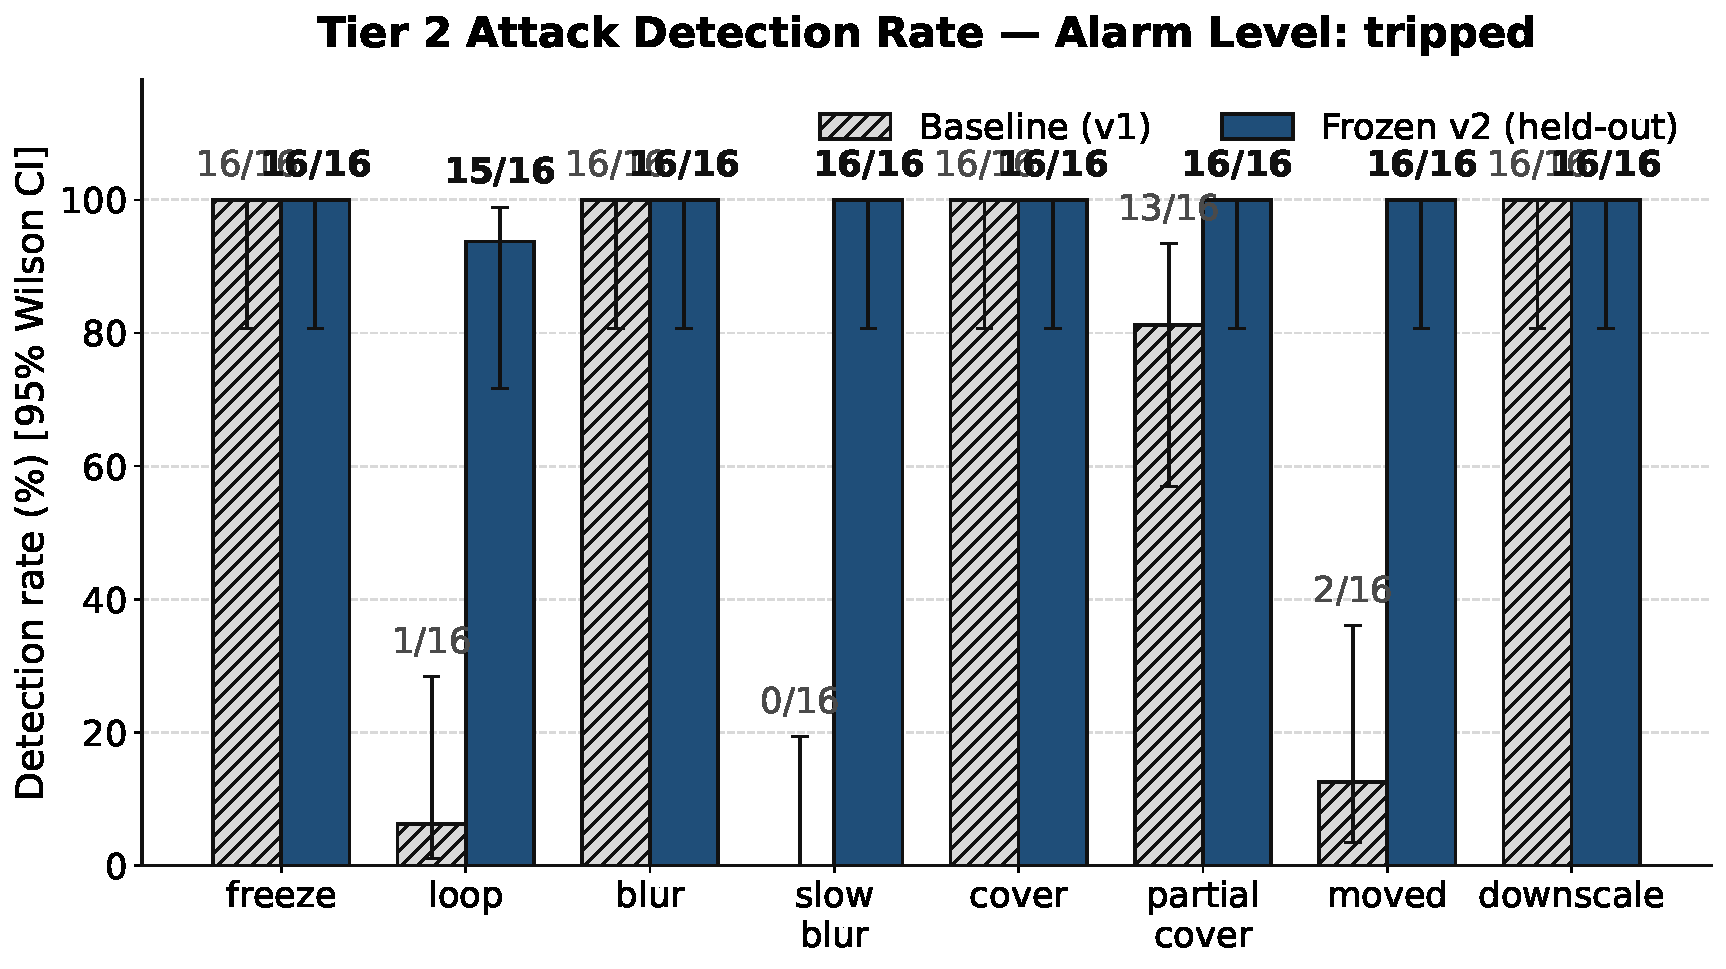
\includegraphics[width=0.92\textwidth]{detection_rate_tripped.pdf}
  \caption{Real CUHK Avenue held-out detection rate comparison at the \texttt{tripped} threshold (\texttt{v1} baseline vs. \texttt{v2} tuned)}
  \label{fig:tripped_rates}
\end{figure}

\begin{figure}[!ht]
  \centering
  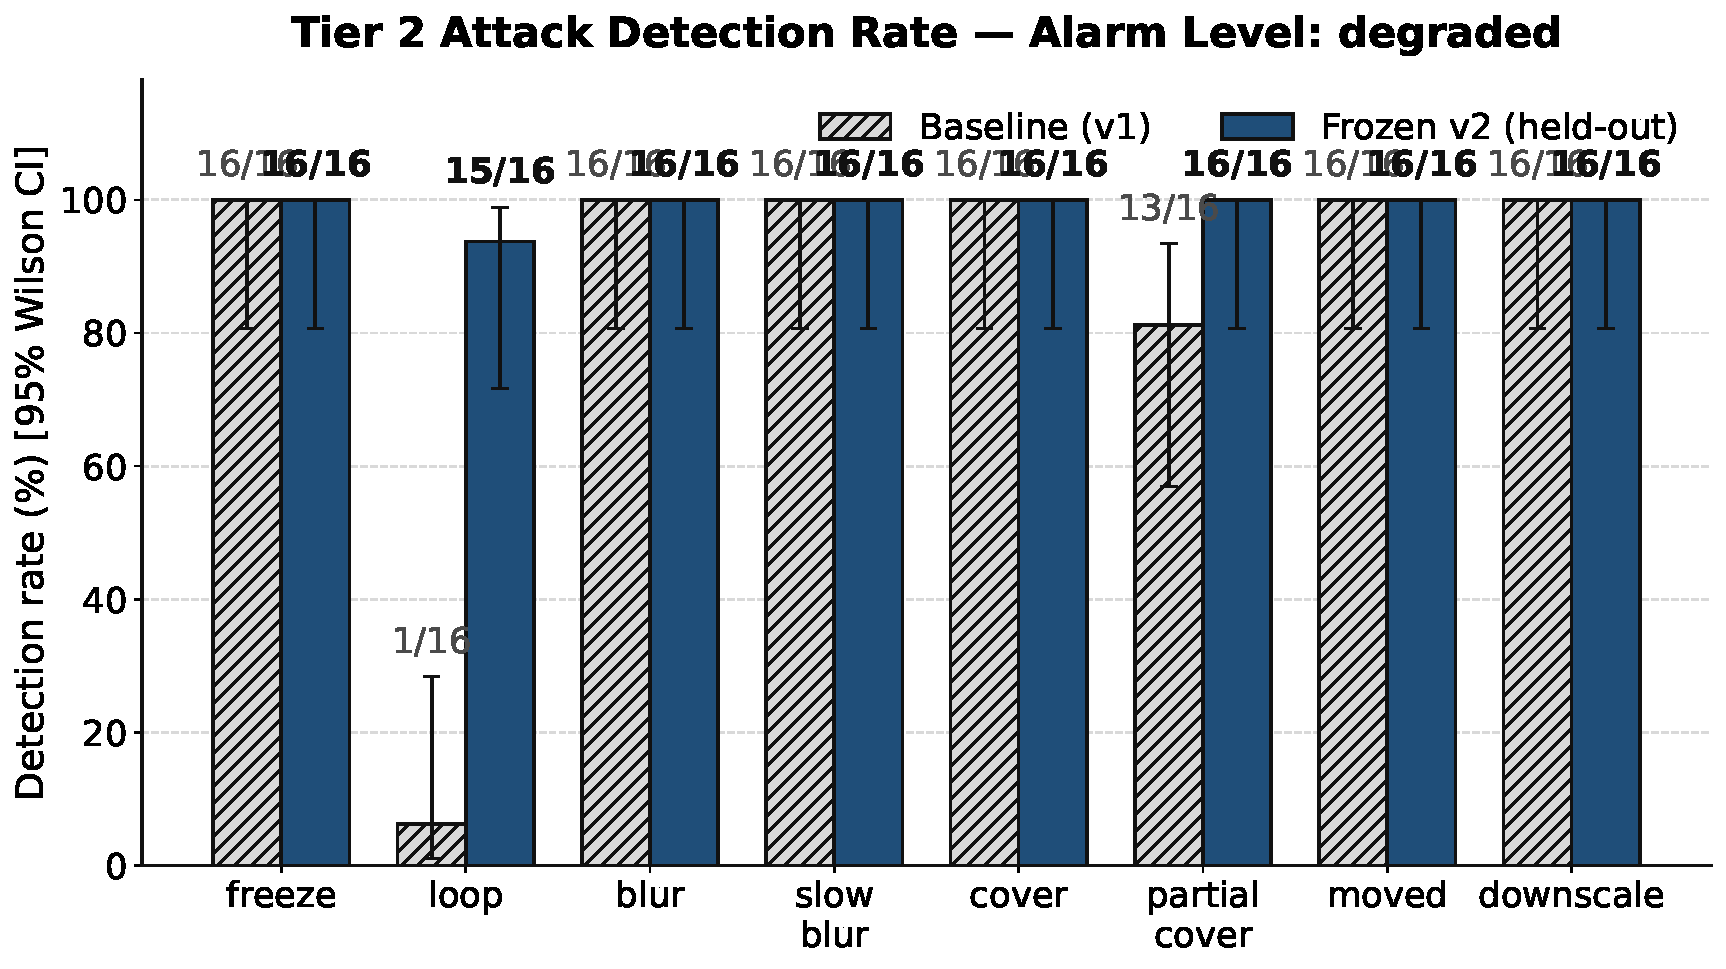
\includegraphics[width=0.92\textwidth]{detection_rate_degraded.pdf}
  \caption{Real CUHK Avenue held-out detection rate comparison at the early \texttt{degraded} warning level}
  \label{fig:degraded_rates}
\end{figure}

\begin{figure}[!ht]
  \centering
  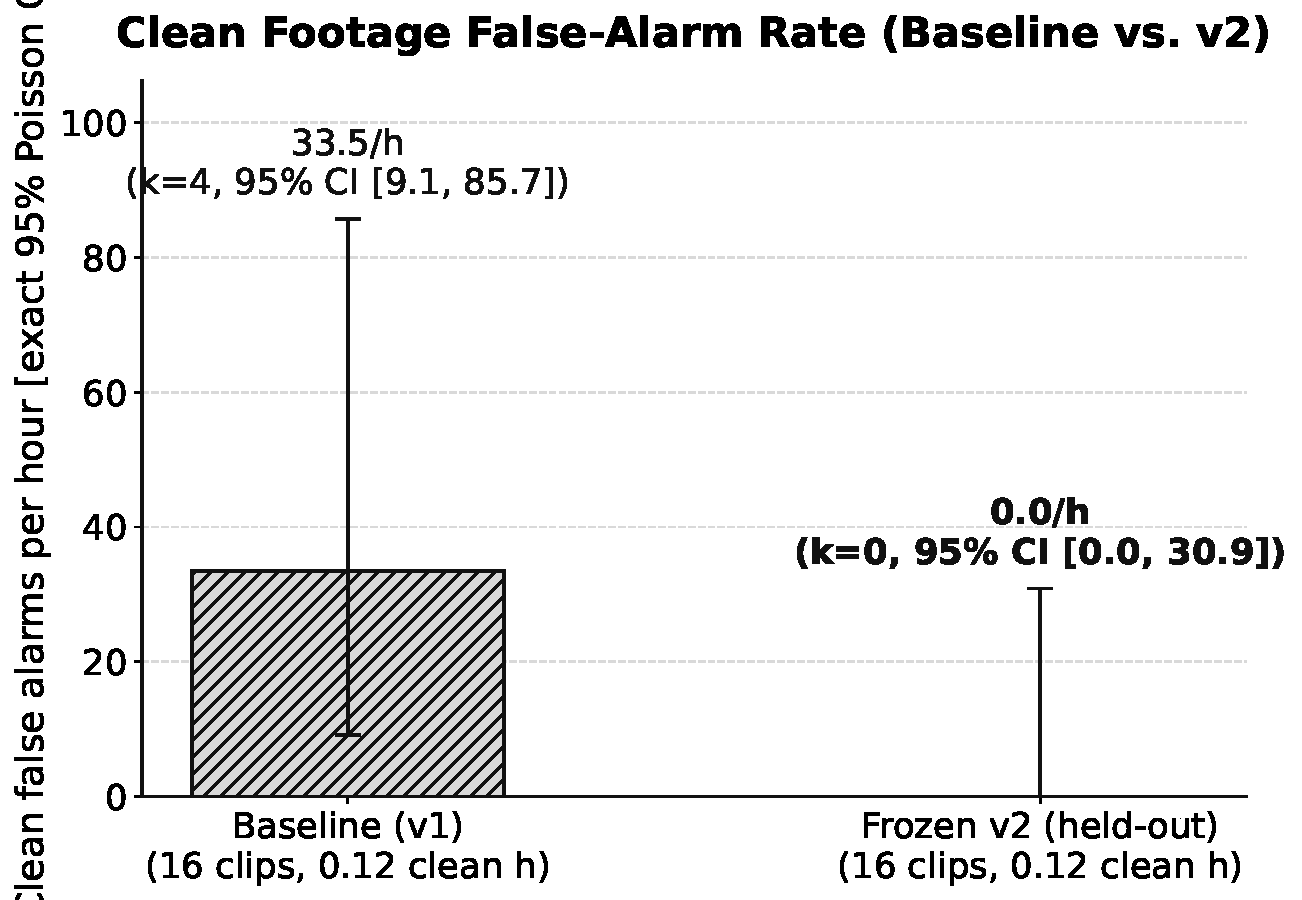
\includegraphics[width=0.78\textwidth]{false_alarms_per_hour.pdf}
  \caption{Clean-footage false alarm rates per hour (with exact 95\% Poisson confidence bounds) on Avenue training and held-out sets}
  \label{fig:fa_rates}
\end{figure}

\subsection{Runtime CPU Throughput Benchmark}
Timed across 300 frames (\texttt{synthetic\_pattern} $320 \times 180$) on an Intel Core i5-12450H CPU using Python~3.12.6 and OpenCV~5.0.0 (\texttt{eval/benchmark\_speed.py}), \texttt{v2} sustains \textbf{281.9~FPS} ($3.55$~ms/frame) at $320$~px width and \textbf{71.2~FPS} ($14.04$~ms/frame) at $640$~px width against \texttt{v1}'s $606.8$~FPS and $84.8$~FPS. Thus, even with full ring-buffer loop checks enabled on CPU alone, \texttt{v2} maintains more than $2\times$ real-time throughput headroom above standard $25\text{--}30$~FPS IP camera streams. Pure-Python IG-DCTF fusion adds minimal overhead ($4.69~\mu$s/call vs. $2.60~\mu$s/call for Channel~A alone, excluding I/O).

\subsection{Synthetic Formula Sanity Check and Ablation (\texorpdfstring{$n = 120$}{n = 120}, Explicitly Labelled Synthetic)}
To verify that the IG-DCTF equation obeys non-compensation and does not degrade posture scoring when Channel~B telemetry is absent, Table~\ref{tab:syn_models} and Figures~\ref{fig:syn_cmp}--\ref{fig:decision_map} summarize results across $120$ hand-authored scenarios ($63$ fabricated, $57$ genuine; $30$ containing Channel~B drift/liveness values, $90$ carrying attribute posture only).

\begin{table}[!ht]
  \centering
  \caption{Synthetic formula sanity check ($n = 120$, positive = \texttt{fabricated}; \textbf{synthetic corpus, not field accuracy})}
  \label{tab:syn_models}
  \begin{tabular}{@{}lccccccccc@{}}
    \toprule
    \textbf{Model / Variant} & \textbf{Acc.} & \textbf{Prec.} & \textbf{Recall} & \textbf{Spec.} & \textbf{$F_1$} & \textbf{TP} & \textbf{FP} & \textbf{TN} & \textbf{FN} \\
    \midrule
    Weighted Average (WA) & 0.7917 & 1.0000 & 0.6032 & 1.0000 & 0.7525 & 38 & 0 & 57 & 25 \\
    Advanced (Channel~A only) & 0.8333 & 1.0000 & 0.6825 & 1.0000 & 0.8113 & 43 & 0 & 57 & 20 \\
    Bayesian Log-Odds & 0.8417 & 0.9400 & 0.7460 & 0.9474 & 0.8319 & 47 & 3 & 54 & 16 \\
    Channel~B only & 0.6250 & 1.0000 & 0.2857 & 1.0000 & 0.4444 & 18 & 0 & 57 & 45 \\
    Additive fusion ($T_{\mathrm{cve}} - 70(1-s)$) & 0.9167 & 1.0000 & 0.8413 & 1.0000 & 0.9138 & 53 & 0 & 57 & 10 \\
    \textbf{IG-DCTF (Multiplicative Gate)} & \textbf{0.9750} & \textbf{1.0000} & \textbf{0.9524} & \textbf{1.0000} & \textbf{0.9756} & \textbf{60} & \textbf{0} & \textbf{57} & \textbf{3} \\
    \bottomrule
  \end{tabular}
\end{table}

Stratification confirms the gate acts selectively: on the $n = 90$ scenarios without Channel~B signals, IG-DCTF identically matches Channel~A ($0.967$ accuracy / $0.966$ $F_1$), whereas on the $n = 30$ Channel-B scenarios, vulnerability-only models sit near chance ($0.433$--$0.467$ accuracy) while IG-DCTF attains $1.000$ (exact McNemar~\cite{mcnemar1947} $17$ vs. $0$ discordant scenarios, $p = 1.53 \times 10^{-5}$). Additive fusion misses $10$ attacks versus $3$ for the multiplicative gate, proving why non-compensation matters. Across 42 threshold pairs, the sweep surface stays flat ($0.9756$ $F_1$ everywhere), meaning thresholds $(0.50, 0.85)$ are justified analytically rather than fitted on data. Synthetic Tier~1 ($13$ distinct drift pairs, $0.0038$~ms/device) and earlier synthetic Tier~2 checks ($80$ runs, $9.6$~frames mean latency) provide regression checks rather than field estimates.

\begin{figure}[!ht]
  \centering
  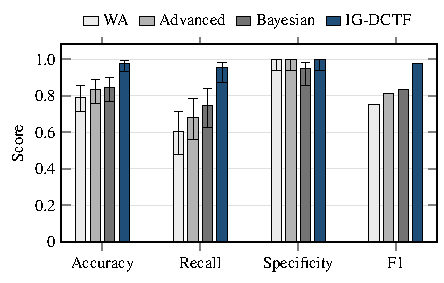
\includegraphics[width=0.88\textwidth]{fig08_comparison.pdf}
  \caption{Synthetic 120-scenario comparison across WA, CVE-only (Advanced), Bayesian, and IG-DCTF (with 95\% Wilson~\cite{wilson1927} bounds)}
  \label{fig:syn_cmp}
\end{figure}

\begin{figure}[!ht]
  \centering
  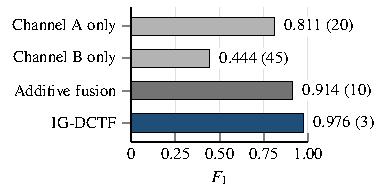
\includegraphics[width=0.78\textwidth]{fig09_ablation.pdf}
  \caption{Ablation on synthetic corpus showing why multiplicative gating avoids linear compensation ($FN = 3$ vs. $10$ additive)}
  \label{fig:ablation}
\end{figure}

\begin{figure}[!ht]
  \centering
  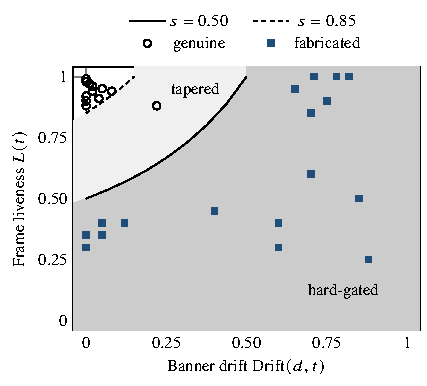
\includegraphics[width=0.72\textwidth]{fig10_decision_map.pdf}
  \caption{IG-DCTF decision regions in the $(\mathrm{Drift}, L)$ plane showing iso-integrity curves at $s = 0.50$ and $s = 0.85$}
  \label{fig:decision_map}
\end{figure}

\chapter{Conclusion and Further Work}

\section{Conclusion}
COBRA-WATCH addresses the blind spot between cyber vulnerability posture and surveillance feed authenticity through Integrity-Gated Dual-Channel Trust Fusion (IG-DCTF). By combining passive vulnerability risk scoring ($T_{\mathrm{cve}}$) with multiplicative signal-integrity gating ($G(s)$), a nominal camera with zero known CVEs is systematically bounded to \texttt{low\_trust} ($T_{\mathrm{final}} \le 30$) whenever its feed integrity drops below $\theta_{\mathrm{low}} = 0.50$, while preserving full tolerance for benign single-field firmware changes.

Within the strict passive legal boundary established for BE Major Project Review~2, the platform demonstrates three grounded results: (i) non-attributive Censys aggregate analysis documenting \textbf{104,218} exposed Indian camera hosts (\textbf{81,285} exposing RTSP port~554) with zero raw target IP redistribution; (ii) frozen \texttt{v2} Tier~2 visual liveness detection on held-out real CUHK Avenue videos raising replay-loop detection from \textbf{1/16} to \textbf{15/16} ($93.8\%$), hitting \textbf{16/16} across seven additional tamper modes (\texttt{freeze}, \texttt{blur}, \texttt{slow\_blur}, \texttt{cover}, \texttt{partial\_cover}, \texttt{moved}, \texttt{downscale}), keeping \texttt{tripped} clean false alarms at \textbf{0.0/h} ([0.0, 30.9]), and executing at \textbf{281.9~FPS} ($320$~px) / \textbf{71.2~FPS} ($640$~px) CPU throughput; and (iii) an end-to-end verified FastAPI + Next.js~16 system with SHA-256 Merkle audit chains, \texttt{/24} IP masking, clear simulated-fixture disclosure, 439 passing backend/pipeline/eval tests (prior to final guard refinement; 16/16 post-guard GNN tests), and 81 passing frontend unit/contract tests.

\section{Limitations and Future Scope}
Transparent reporting requires stating four open boundaries planned beyond Review~2:
\begin{enumerate}
  \item \textbf{Longitudinal Tier~1 Field Evaluation:} Because Censys history access spans multi-month time series, empirical false-positive rates for passive banner drift between legitimate firmware upgrades and proxy substitutions remain future scope.
  \item \textbf{Owned Laboratory Camera Testbed:} Real-footage Avenue validation relies on programmatic tamper onset over $0.1195$~h of clean held-out video (producing a wide Poisson upper CI of $30.9$/h). Recording long-duration un-tampered and physically tampered RTSP streams on owned laboratory IP cameras---including day/night lighting transitions---will narrow false-alarm bounds.
  \item \textbf{Adaptive Evasion Analysis:} While \texttt{v2} catches frame replays carrying natural scene motion, an adaptive adversary injecting subtle per-frame sensor noise to bypass perceptual-hash matching remains open for adversarial hardening.
  \item \textbf{Scalable Production Backend:} Single-writer SQLite suits single-node Review~2 demonstration and evaluation scale; high-concurrency enterprise deployment requires migrating to PostgreSQL and horizontally scalable worker queues.
\end{enumerate}


\addcontentsline{toc}{chapter}{References}
\renewcommand{\bibname}{References}\thispagestyle{plain}

\bibliographystyle{ieeetr}
\bibliography{san}

\newpage
\begin{center}
  \vspace*{10cm}
  \centering
  {\huge \bfseries Appendices}
\end{center}

\let\cleardoublepage\clearpage
\appendix

\chapter{Weekly Progress Report}
\noindent\textbf{[TODO — Team / Ankita]:} Insert scanned pages or table exports of the signed semester Weekly Progress Report sheet here before final PDF export (replace this notice with image figures of the signed pages).
% Example once image/PDF is added to report/figures/:
% \begin{figure}[h]
%   \centering
%   \includegraphics[width=0.9\textwidth]{weekly-progress.pdf}
%   \caption{Signed Weekly Progress Report}
%   \label{fig:weekly_progress}
% \end{figure}

\newpage
\chapter{Plagiarism Report}\thispagestyle{plain}
\noindent\textbf{[TODO — Lead / Guide]:} Attach the official plagiarism check summary PDF/screenshot approved by the supervisor and project co-ordinator before final Review 2 submission.
% Example once plagiarism-report.pdf is placed in report/figures/:
% \usepackage{pdfpages} % add to preamble if including multi-page PDF
% \includepdf[pages=-,pagecommand={},width=\textwidth]{figures/plagiarism-report.pdf}

\newpage
\chapter{IPR Status}
\begin{enumerate}
  \item \textbf{Research Paper in Preparation:} ``Integrity-Gated Dual-Channel Trust Fusion for OSINT-Discovered Surveillance Cameras'' (manuscript sources in \texttt{paper/main.tex}; not yet submitted).
  \item \textbf{Censys Research Access Ticket RS-469:} Approved academic/research access used strictly as evidence of real non-attributive aggregate metadata collection (\texttt{data/censys/2026-11-26/snapshot.json}; zero raw IPs persisted or published).
  \item \textbf{Code Repository:} Version-controlled platform source, evaluation harness, and reproducible snapshot tools hosted at \url{https://github.com/Gokul0211/Geospatial-Camera-Exposure-Intelligence-Platform}.
\end{enumerate}

\begin{acknowledgments}\thispagestyle{plain}
\addcontentsline{toc}{chapter}{Acknowledgement}
We take this opportunity to express our profound gratitude and deep regards to our guide \textbf{[TODO: Miss Gaikwad Full Name]} and project coordinator \textbf{[TODO: Project Co-ordinator Name]}, for their exemplary guidance, constant encouragement, and valuable supervision throughout the completion of this project. Their mentorship has been invaluable in enhancing our understanding of the various concepts and technical skills required to successfully complete our work. The blessings, help, and guidance given by them from time to time shall carry us a long way in the journey of life on which we are about to embark.

We also take this privilege to express our sincere thanks to Dr. Mukesh D. Patil, Principal, Ramrao Adik Institute of Technology (RAIT), D. Y. Patil Deemed to be University, for providing the necessary facilities and academic environment conducive to research and innovation. We are equally thankful to Dr. A. V. Vidhate, Head of the Department of Computer Engineering, for his constant support and motivation. Last but not least, we would also like to thank all those who have directly or indirectly helped us in the successful completion of this project report.
\end{acknowledgments}

\end{document}
